\documentclass[]{article}
\usepackage[round]{natbib}

\usepackage{fullpage}
\usepackage[parfill]{parskip}
\usepackage{listings}
\usepackage{url}
\usepackage{authblk}
\usepackage{graphicx}
\usepackage{xcolor}
\usepackage{booktabs}
\usepackage{amsmath}

\lstset{language=Python}

% local definitions
\newcommand{\comment}[1]{{\textcolor{red}{Comment: #1}}}
\newcommand{\aprcomment}[1]{{\textcolor{blue}{APR: #1}}}
\newcommand{\krtcomment}[1]{{\textcolor{purple}{KRT: #1}}}
\newcommand{\krtedit}[2]{{\emph{\textcolor{gray}{#1}}}{\textcolor{purple}{#2}}}
\newcommand{\apredit}[2]{{\emph{\textcolor{gray}{#1}}}{\textcolor{blue}{#2}}}

\usepackage{xspace}
\newcommand{\GEVA}{\texttt{GEVA}\xspace}
\newcommand{\tsdate}{\texttt{tsdate}\xspace}
\newcommand{\relate}{\texttt{Relate}\xspace}

% cross-reference with supplement
\usepackage{xr}
\externaldocument{supplement}

\title{Multiple sources of uncertainty confound inference of
historical human generation times}
\author[1,*]{Aaron P. Ragsdale}
\author[2]{Kevin R. Thornton}
\affil[1]{University of Wisconsin--Madison, Wisconsin, USA}
\affil[2]{University of California, Irvine, California, USA}
\affil[*]{apragsdale@wisc.edu}

\begin{document}
\maketitle

\begin{abstract}

    \noindent \citet{wang2023human} recently proposed an approach to infer the
    history of human generation intervals from changes in mutation profiles
    over time. As the relative proportions of different mutation types depend
    on the ages of parents, binning variants by the time they arose allows for
    the inference of average paternal and maternal generation intervals over
    times. Applying this approach to published allele age estimates,
    \citet{wang2023human} inferred long-lasting sex differences in average
    generation times and surprisingly found that ancestral generation times of
    West African populations remained substantially higher than those of
    Eurasian populations extending tens of thousands of generations into the
    past. Here we argue that the results and interpretations in
    \citet{wang2023human} are primarily driven by noise and biases in input
    data and a lack of validation using independent approaches for estimating
    allele ages. With the recent development of methods to reconstruct
    genome-wide gene genealogies, coalescence times, and allele ages, we
    caution that downstream analyses may be strongly influenced by
    uncharacterized biases in their output.

\end{abstract}

Recent years have seen the rapid development of methods for reconstructing
genetic genealogical structures of large unrelated cohorts
\citep{speidel2019method,wohns2022unified,hubisz2020mapping}, which are
comprised of a series of gene genealogies (or trees) along the genome.
Reconstructed genealogies (or informative summaries of them) have the potential
to transform population genetic inference. Biological and evolutionary
processes determine the structure of these genealogies, including the
distribution of mutations. In particular, the age of a variant can be estimated
by mapping its mutation to the branch of the genealogy consistent with the
observed data.

The past few years have also seen efforts to sequence large sets of pedigrees,
providing increased resolution of important parameters of genome biology such
as direct measurements of mutation rates and profiles. Through high-coverage
sequencing of multiple generations of families, \emph{de novo} mutations can be
determined as maternally or paternally inherited. With a large enough sample
size (meoises), both the number of mutations and proportions of mutation types
(i.e., the \emph{mutation spectrum} of A$\rightarrow$C, A$\rightarrow$G, etc.\
mutation types) can be correlated with parental age and sex
\citep{jonsson2017parental,halldorsson2019characterizing}. These two sets of
inferences, the estimated ages of mutations and the parental age- and
sex-dependence of the mutation spectrum, can be combined to infer the history
of average maternal and paternal generation intervals for human populations of
diverse ancestries \citep{macia2021different,wang2023human}. In order to avoid
overfitting, this approach requires making a number of assumptions about the
constancy of the mutational process over time and its similarity across
populations \citep{harris2015evidence,mathieson2017differences,harris2017rapid,
dewitt2021nonparametric}, and of negligible effects of selection and biased
gene conversion \citep{lachance2014biased,glemin2015quantification} on shaping
the profile of segregating mutation types.

\cite{gao2023limited} have recently criticized this approach.
They show that observed changes in the mutation spectrum over
time cannot be explained by changes in maternal and paternal generation
intervals alone. Male and female generation
times are required to change in different directions within the same time interval in
order to explain the data for different classes of mutation.
They argue that factors other than changes in generation intervals,
including genetic modifiers and environmental exposure, must explain observed
variation in mutation profiles.
\citet{gao2023limited} also point out that pedigree-based estimates of the
\emph{de novo} mutation spectrum do not agree with the mutation spectrum among
young variants in existing population-level datasets,
potentially biasing such approaches. Because such mutations
occurred recently, these discrepancies would require strong mutation-type-specific
selection or large recent shifts in the \emph{de novo} mutation spectrum.

In this note, we examine both the results and conclusions of
\citet{wang2023human}. We first consider the reported inferred generation time
histories and find that they are inconsistent with current understanding of
human population history, in particular population structure within Africa. In
exploring the source of this inconsistency, we show that allele age estimates
are not just noisy, but age-stratified mutation spectra reconstructed using
independent methods do not agree, with mutation profiles diverging in opposing
directions. Thus, the results from \citet{wang2023human} do not reproduce
when applying different estimates of allele ages from the same population samples. We
further discuss the disagreement between the mutation rate profile found in
pedigree studies and from young variants, the source of which is not well
understood and complicates their comparison. In conclusion, we suggest that
current methods of genealogical reconstruction and allele age estimation
should continue to be evaluated for subtle biases, and that
downstream analyses using estimated allele ages and mutation profiles should
carefully validate their results.

\subsection*{Long-lasting differences in population-specific generation intervals}

Applying the proposed inference approach to multiple populations of different
continental ancestries, \citet{wang2023human} estimated that the ancestors of
European, East Asian, and South Asian populations included in the
\citet{1000genomes2015} dataset (1KGP) have a history of significantly reduced
average generation times compared to West African populations. These
differences extend to over 10,000 generations, the time period highlighted in
their study.
In discussing this inference the authors state, ``[T]he difference
among populations beyond 2000 generations ago reflects population structure in
humans before their dispersal out of Africa, a structure that is not fully
captured by the 1000 Genomes AFR sample. This implies that the simple labels of
`African' and `non-African' for these populations conceal differences in
generation times that existed on our ancestral continent.'' Indeed, a number of
recent genetic studies suggest that human population structure within Africa
extending hundreds of thousands of years into the past has shaped
present-day genetic variation
\citep{hammer2011genetic,hsieh2016model,hey2018phylogeny,
ragsdale2019models,lorente2019whole,durvasula2020recovering}.

\begin{figure}[t!]
    \centering
    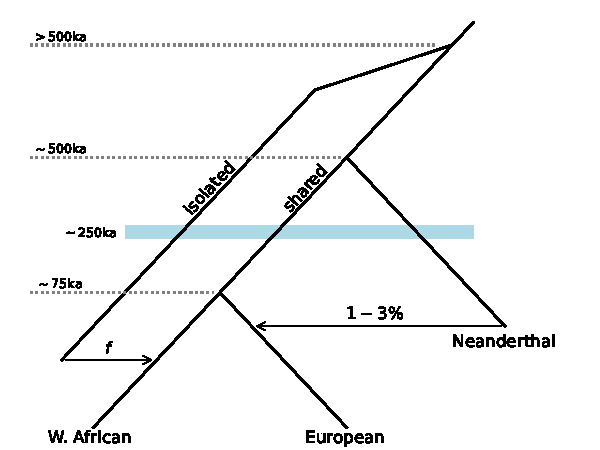
\includegraphics[width=0.5\textwidth]{../plots/durvasula_model}
    \caption{
        \textbf{A model for archaic admixture within Africa.} In such a model
        for ``ghost'' archaic introgression within Africa
        \citep{durvasula2020recovering}, an isolated lineage diverged prior to
        the human-Neanderthal split and more recently contributed ancestry
        (with proportion $f$) to West African, but not European populations.
        The mutation spectrum of West African populations among alleles dating
        to $\sim250-300$ka is due to a combination of mutations from the
        ``shared'' and ``isolated'' lineages, while the European populations'
        spectrum from this time is due to a combination from the ``shared'' and
        Neanderthal branches.  \citet{wang2023human} showed that masking
        Neanderthal segments in Eurasian populations had a negligible effect on
        their inferred generation time histories, so we ignore this small
        contribution when comparing observed mutation spectra between West
        African and Eurasian groups.
    }
    \label{fig:durvasula-model}
\end{figure}

However, in extending their analysis deeper into the past,
\citet{wang2023human} find that ancestral generation intervals do not converge
until many 10s of thousands of generations ago. Assuming an average generation
time of 25--30 years, this corresponds to one to two million years in the past.
This observation would require some portion of the ancestries of Eurasian and
West African populations to have remained isolated for many hundreds of
thousands of years, for those structured ancestral populations to have had
large differences in average generation times over the course of this history,
and for those groups to have contributed substantively to different
contemporary human populations. While such a scenario of long-lasting isolation
among ancestral populations is not impossible, it is not supported by genetic
\citep[e.g.,][]{ragsdale2022weakly} or archaeological
\citep[e.g.,][]{scerri2018did} evidence, which rather suggest at least periodic
connectivity of ancestral human populations within Africa.

Genetic studies have estimated the Eurasian--West African divergence (i.e., the
time of recent shared ancestry) at only $\approx 75$ka (thousand years ago)
\citep[e.g.,][]{pagani2015tracing,bergstrom2020insights}. While population
genetic studies vary considerably in estimated split times, even those that
infer deeper human divergences place the Eurasian--West African divergence at
100--150ka \citep[e.g.,][]{schlebusch2017southern}. If such estimated
divergence times represent the majority of ancestry of the two groups (while
allowing for a smaller portion to be due to long-lasting structure), then the
shared portion of ancestry should be subject to the same generation intervals
prior to the divergence time. Any differences in the mutation spectrum from
those epochs would be driven by differences in generation times affecting the
minority of ancestry that remained isolated. 

As a simple test of such a scenario, we considered a model of archaic admixture
within Africa, allowing for some proportion of admixture from a diverged
lineage into West African populations (such as $\approx10\%$ as inferred by
\citet{durvasula2020recovering}, Figure~\ref{fig:durvasula-model}). At 10,000
generations ago, average paternal and maternal generation intervals in the
ancestors of Eurasians were inferred to both be $\approx20$ years, while the
ancestral African generation intervals were at least 28 and 23 (see Figure S4
in \citet{wang2023human}). Using the same mutation model
\citep{jonsson2017parental}, we can determine the generation intervals in the
isolated lineage that is needed to result in a mutation spectrum matching that
of the inferred generation times (see Supporting Information).

We assume that admixture proportions from the diverged and Eurasian-shared
lineages ($f$ and $1-f$, respectively) result in surviving variation from those
epochs having similar proportions of contributions (in effect, ignoring
differences in total mutation rate and demographic effects that may distort
the magnitude of the contributed mutation spectra, see Supporting Information).
With 10\% admixture into the ancestors of West Africans from a diverged
lineage, the mean paternal age of conception would need to be 92 and the mean
maternal age 48.  These are unreasonably long generation times for \emph{Homo}
species. With 20\% admixture from this diverged lineage (which is larger than
has been proposed or inferred in previous genetic studies), mean ages would
still need to be 58 and 34. For the paternal average generation time to be less
than 40, this model would require $f=0.4$ or that the inferred generation times
in the shared branch were considerably higher
(Table~\ref{tab:structured-ages}).

Therefore, even assuming a model of long-lasting population structure with
strict isolation within Africa, we find the reconstructed generation time
intervals over the past 10,000 years from \citet{wang2023human} to be
incompatible with plausible life histories of early humans. Given this, it is
natural to ask what may be causing such mis-inference. Below we show that
multiple sources of uncertainty, namely noise and bias in allele age inference
and inconsistencies in trio-base estimates of mutation profiles, confound
inferences of generation times from age-stratified mutation spectra.

\subsection*{Inconsistencies in inferred mutation spectra over time}

\citet{wang2023human} used
published allele ages from \GEVA \citep{albers2020dating}
to construct mutation spectra within time periods. \GEVA estimates
allele ages by considering the number of mutations that have accumulated on the
ancestral haplotype carrying the focal variant, as well as the effect of
recombination in reducing the size of that ancestral haplotype. Singletons are
excluded from analysis and are not assigned an age. Partitioning variants by
their estimated ages shows that the mutation spectrum has changed over time,
assuming that the observed spectrum of segregating variation is not biased with
respect to the spectrum of \emph{de novo} mutations occurring during that time
(Figure~\ref{fig:spectrum-ages}A and see Figure 1C in \citet{wang2023human}).

\begin{figure}[t!]
    \centering
    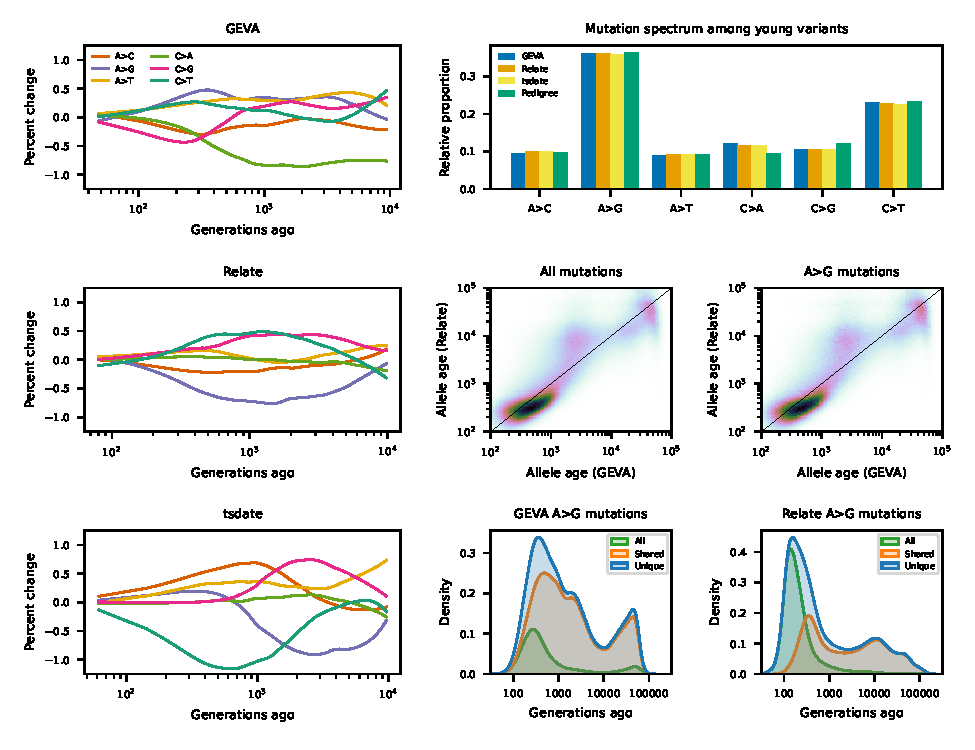
\includegraphics{../plots/fig1.pdf}
    \caption{
        \textbf{Time-stratified mutation spectra are inconsistent and poorly
        fit by historical generation time changes.} (A-C) Three methods for
        estimating allele ages provide incongruous mutation spectrum histories.
        (D-F) In fitting historical generation intervals to each observed
        mutation spectrum profile, none of the mutation spectrum histories
        observed in the data are recovered by the predicted spectra using the
        inferred generation time histories. Trajectories are smoothed using
        LOESS regression.
    }
    \label{fig:spectrum-ages}
\end{figure}

In fitting generation time histories to data from the past 10,000 generations,
we find that the inferred generation times provide a poor fit to the data
(Figure~\ref{fig:spectrum-ages}D). The relative proportions of the predicted
mutation spectrum trend in opposite directions for some mutation classes,
confirming the concern from \citet{gao2023limited} that a single generation
time history cannot simultaneously explain each of the six mutation class
frequency changes. For alleles older than 10,000 generations, the mutation
spectrum fluctuates by large amounts (Figure~\ref{fig:geva-spectra-80k}). While
estimated allele ages from the distant past have decreased accuracy
\citep{albers2020dating,wang2023human}, the large differences in proportions
suggests a bias in \GEVA's reported dates that correlates with mutation type.

Accurate dating of variant ages is central to the inference of generation
intervals from time-stratified mutation spectra.
Given the poor fit of the model to the \GEVA data and the known uncertainty in
age estimation for older variants, we attempted to reproduce the inferred
generation time histories using allele age estimates from independent sources,
\relate \citep{speidel2019method} and \tsdate \citep{wohns2022unified}, both
state-of-the-art genealogical reconstruction methods able to scale to modern sample sizes. 
The ages of variants
dated by at least two of the methods are only moderately correlated (\GEVA and
\relate: $r^2 \approx 0.28$, \GEVA and \tsdate: $r^2 \approx 0.33$, \tsdate
and \relate: $r^2 \approx 0.64$; Figure~\ref{fig:data-comp}A-C and see Figure
S20 from \citet{wohns2022unified}). Imperfect correlations should be expected,
as genealogical reconstruction methods have been shown to vary in the accuracy
of estimated $T_{MRCA}$ \citep{brandt2022evaluation}.

\begin{figure}[t!]
    \centering
    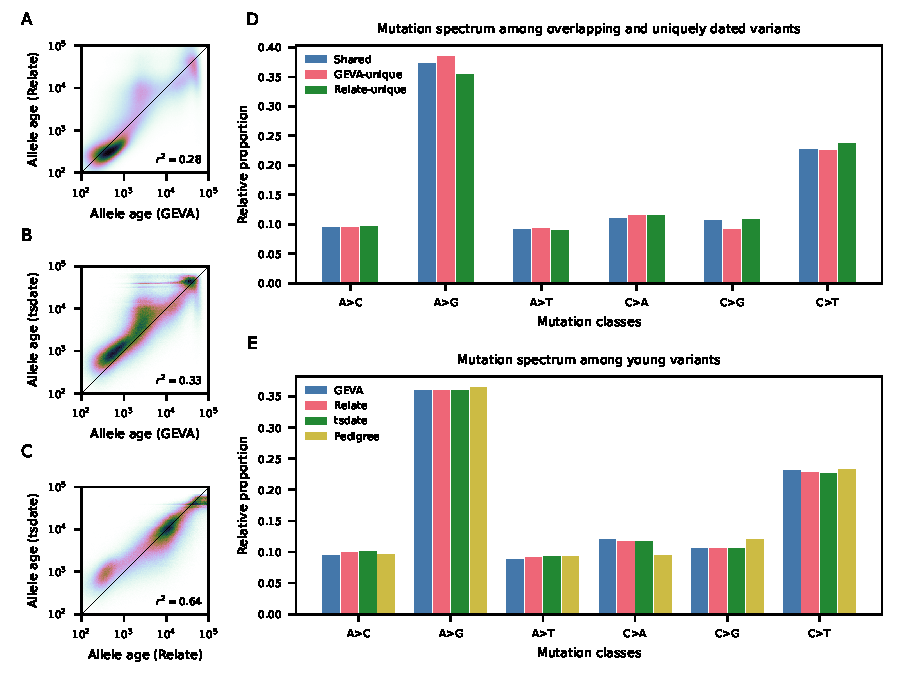
\includegraphics{../plots/fig2.pdf}
    \caption{
        \textbf{Comparing allele ages and mutation spectra across data
        sources.} (A-C) Allele age estimates are only moderately correlated
        between methods. Shown here are allele age estimates for variants that
        were assigned ages by two or more of \GEVA, \relate and \tsdate. (D)
        The proportions of mutation types uniquely dated by \GEVA and \relate
        differ from the variant proportions among mutations dated by both
        methods, indicating biases in the mutation types that are kept and
        discarded. Here, we compared \GEVA and \relate (instead of \tsdate)
        because allele ages were obtained from the same input data, namely
        phase three of the 1KGP.
        (E) While the mutation spectrum among young variants dated
        to $<100$ generations is similar between age estimation methods,
        the pedigree-based estimate of the \emph{de novo} mutation spectrum
        \citep{jonsson2017parental} differs, in particular for C$\rightarrow$A
        and C$\rightarrow$G mutations.
    }
    \label{fig:data-comp}
\end{figure}

Despite the imperfect correlation, it is still possible that differences in
estimate allele ages are unbiased with respect to mutation type.
However, we find that ages provided by each method disagree
at the level of individual mutation
spectrum histories (Figures~\ref{fig:spectrum-ages}A-C and
\ref{fig:geva-spectra}--\ref{fig:tsdate-spectra}), with 
changes in mutation proportions
often trending in opposite directions over the same time periods. In
turn, these divergent spectrum histories provide qualitatively different
inferred generation time histories
(Figures~\ref{fig:geva-gen-times}--\ref{fig:tsdate-gen-times}). None
of them provide a reasonable fit to the data (Figure
\ref{fig:spectrum-ages}D-F).

Published allele ages from both \citet{albers2020dating} (\GEVA) and
\citet{speidel2019method} (\relate) used the same input dataset: the phase 3
release of 1KGP. However, they differ in the total number of variants that were
assigned ages (roughly 30 million and 48 million, respectively). \GEVA and
\relate each discard variants that violate or are inconsistent with certain
assumptions, such as allowing only a single mutation at a given site,
while \tsdate retains all data by allowing for multiple mutations at a site.
Of those variants, 25 million variants were dated by both \GEVA and \relate,
with the remaining uniquely
assigned an age by one or the other method. When comparing mutation spectrum
histories restricted to variants dated by both \GEVA and \relate, the two
methods still predict different mutation profile trajectories
(Figure~\ref{fig:overlap-spectra}). In comparing the proportions of mutation
types assigned ages by both methods or uniquely by one, we find that those
proportions differ considerably (Figure~\ref{fig:data-comp}D). For example,
\GEVA provides age estimates for relatively more A$\rightarrow$G mutations and
fewer C$\rightarrow$G mutations, while \relate provides age estimates for
relatively more C$\rightarrow$T and fewer A$\rightarrow$G mutations. This owes
to methodological differences in evaluating whether a particular variant can be
reliably dated, which may have both bioinformatic (e.g., genotyping and phasing
errors) and biological (e.g., recurrent mutations) causes. Therefore, when
comparing mutation spectra that are conditioned on variants being dated by a
particular method, it is not apparent which method, if any, provides unbiased
estimates of age-stratified mutation spectra.

\subsection*{Mutation spectra differ between \emph{de novo} mutations and young
alleles}

The large disagreements in mutation spectrum histories between multiple variant
age-estimation methods are concerning for downstream inferences that rely on
them. Independent of biases in allele age estimate, there are further problems
in comparing age-stratified mutation spectra to those estimated from pedigree
studies \citep{jonsson2017parental,halldorsson2019characterizing}. As
\citet{wang2023human} acknowledge, the spectrum of \emph{de novo} mutations
identified in Icelandic trios \citep{jonsson2017parental} differs from the
spectrum of young segregating variation (e.g., variants estimated to be less
than 100 generations old, Figure~\ref{fig:data-comp}E and
Table~\ref{tab:recent-spectra}). \citet{gao2023limited} argue that these
differences are unlikely to be driven by biological processes.

For some mutation classes, the relative proportion of \emph{de novo} mutations
in the trio-based study differs from the young-variant spectrum by up to
$0.02$, which would imply a large over- or under-count of different mutation
types. This is the equivalent of 10s of thousands of SNPs in the most recent
bin, with the exact number depending on the variant-dating method.
\GEVA, \tsdate and \relate, while their estimated mutation spectra differ at
older times, closely agree for mutations inferred to be less than 100
generations old (Table~\ref{tab:recent-spectra}). In discussing this
discrepancy, \citet{wang2023human} state, ``We found that the mutation spectrum
from the large pedigree study consistently differed from the variant spectrum
inferred from the 1000 Genomes Project data, possibly because we removed
singletons from the polymorphism dataset to reduce errors.'' However, \GEVA does
not provide estimates of allele ages for singletons, so this suggested source
of discrepancy cannot be checked with their published allele ages. Both \tsdate
and \relate report allele ages for singletons, and their inclusion does not
strongly affect the mutation spectrum for very young variants
(Table~\ref{tab:recent-spectra}), though it does impact the mutation profiles
in older time periods (Figures~\ref{fig:relate-spectra-singletons},
\ref{fig:tsdate-spectra-singletons}). Reported ages from \GEVA and \relate both
used the low-coverage phase 3 1KGP data while \tsdate used the more recent
independently sequenced high-coverage 1KGP data \citep{byrska2022high}, so the
accuracy of the mutation spectrum among young variants is unlikely to be driven
by differences in coverage.

To account for the differences between the \emph{de novo} spectrum from
pedigree studies \citep{jonsson2017parental} and the spectrum among young
variants, \citet{wang2023human} subtracted this difference from each historical
mutation spectrum. ``[This choice] has the effect of assuming that parental ages
in the pedigreed mutation dataset reflect generation times in the most recent
historical bin'' \citep{wang2023human}. However, the average generation time
among present-day Icelanders may not reflect average generation times in
world-wide populations over the past 3-5 thousand years, represented by the
most recent time bin in their analysis. Still more concerning is that we do not
know the source of the discrepancy between the Iceland and 1KGP mutation
spectra. Without knowing this, it is unclear that simply subtracting the
differences between them properly accounts for it. Instead, mutation
class-specific genotyping differences may distort the underlying mutation
model, potentially driving deviations in predicted mutation profiles in
unexpected ways.

What could be driving the large disagreement between the spectrum of \emph{de
novo} mutations from Icelandic pedigrees and that of young variants in the 1KGP
dataset? First, there could be true differences in the mutation spectrum
between the Iceland cohort and 1KGP populations, although this seems unlikely, as
populations of different ancestries in 1KGP have more similar recent mutation
spectra to each other than to the Iceland \emph{de novo} spectrum (including
the EUR populations, Table~\ref{tab:population-spectra}). If the differences
are real, then the Icelandic pedigree data is an inappropriate calibration for
the mutation spectrum in other populations. Second, there could be differences
in selective pressures between mutations of different classes, although
selection would need to be very strong for some classes compared to others in
order to see the observed difference among young variants.  Third, the signal
may be driven by genotyping error or bioinformatics choices, though the
agreement between high- and low-coverage 1KGP datasets suggests that genotyping
error does not have a strong effect in the 1KGP data. Instead, filtering and
bioinformatics choices in the pedigree approach are the likely culprit
\citep{bergeron2022mutationathon}. Until the source of these differences are
understood and properly accounted for, we caution that
population-genetic inferences should
avoid calibration using mutation rates and profiles from pedigree studies.

\subsection*{Conclusions}

Large-scale reconstruction of gene genealogies, dating mutations, and
$T_\text{MRCA}$ inference are all exciting developments, but these methods are
quite new and will likely advance considerably in the coming years. Currently,
existing methods show different accuracies even under overly-idealized
conditions \citep{brandt2022evaluation}. We should therefore be cautious of
unexpected and subtle biases that can impact downstream analyses. In the case
of generation time inference \citep{wang2023human}, we showed that patterns of
variation that were attributed to biological processes (variation in generation
times) are predominantly driven by nonbiological artifacts in the input data.
As the field continues to evaluate the accuracy of allele age estimation and
genealogical reconstruction methods, we recommend that analyses that rely on
their output thoroughly validate their results using independent approaches.

\bibliographystyle{genetics}
\bibliography{doc}

\end{document}
